%%%%%%%%%%%%%%%%%%%%%%%%%%%%%%%%%%%%%%%%%%%%%%%%%%%%%%%%%%%%%%%%%%%%%%%%%%%%%
% Seminario 14 del Doble Grado: Resolución del problema Fibonacci GCD
%
% Repositorio del Doble Grado: https://github.com/dgiim/
%
% Trabajo desarrollado a partir de la plantilla de Matemáticas:
% https://github.com/andreshp/PlantillasLatex/tree/master/PlantillaMatematicas
%
%%%%%%%%%%%%%%%%%%%%%%%%%%%%%%%%%%%%%%%%%%%%%%%%%%%%%%%%%%%%%%%%%%%%%%%%%%%%%

%----------------------------------------------------------------------------------------
%	PAQUETES Y OTRAS CONFIGURACIONES DEL DOCUMENTO
%----------------------------------------------------------------------------------------

\RequirePackage[l2tabu, orthodox]{nag}  % Produce un warnig en caso de usar un comando obsoleto.

\documentclass{article}

% Paquetes para el diseño de página:
\usepackage{fancyhdr}                   % Utilizado para hacer títulos propios.
\usepackage{lastpage}                   % Referencia a la última página. Utilizado para el pie de página.
\usepackage{extramarks}                 % Marcas extras. Utilizado en pie de página y cabecera.
\usepackage[parfill]{parskip}           % Crea una nueva línea entre párrafos.
\usepackage[margin=3cm]{geometry}       % Asigna la "geometría" de las páginas.
\usepackage{lipsum}                     % Texto dummy. Quitar en el documento final.

% Fuente utilizada. Elija uno de ellos:
\usepackage{courier}                    % Fuente Courier.
%\usepackage{fourier}                   % Fuente Adobe Utopia.
\usepackage{microtype}                  % Mejora la letra final de cara al lector.

% Paquetes para imágenes:
\usepackage[usenames,dvipsnames]{color} % Permite crear colores propios. Utilizado para el bg de Minted.
\usepackage{graphicx}                   % Utilizado para insertar gráficos.

% Paquetes para matemáticas:                     
\usepackage{amsmath,amsthm,verbatim,amssymb,amsfonts,amscd} % Teoremas, fuentes y símbolos.

% Paquetes para algoritmos:
\usepackage{algpseudocode}
\usepackage{algorithmicx}
\usepackage{algorithm}

% Paquetes para tablas:
\usepackage{booktabs}

% Paquetes para introducir hipervínculos:
\usepackage{hyperref}
\hypersetup{
     colorlinks   = true,
     urlcolor     = cyan
}

% Paquetes para adaptar Látex al Español:
\usepackage[spanish,es-noquoting, es-tabla, es-lcroman]{babel} % Cambia 
\usepackage[utf8]{inputenc}                                    % Permite los acentos.
\selectlanguage{spanish}                                       % Selecciono como lenguaje el Español.

% Estilo de página:
\pagestyle{fancy}                      % fancy
\fancyhf{}                             % Limpia la cabecera y el pie de página.
\geometry{left=3cm,right=3cm,top=3cm,bottom=3cm,headheight=1cm,headsep=0.5cm} % Márgenes y cabecera.

% Espacios en el documento:
\linespread{1.1}                        % Espacio entre líneas.
\setlength\parindent{0pt}               % Selecciona la indentación para cada inicio de párrafo.

% Cabecera del documento:
\renewcommand\headrule{                 % Se ajusta la línea de la cabecera.
\begin{minipage}{1\textwidth}           % Elija una de las siguientes líneas:
%    \hrule width \hsize \kern 1mm \hrule width \hsize height 2pt 
    \hrule width \hsize 
\end{minipage}
}
\lhead{\autor}                          % Parte izquierda.
\chead{}                                % Centro.
\rhead{\titulo}                         % Parte derecha.

% Pie de página del documento:
\renewcommand\footrule{                                 % Se ajusta la línea del pie de página.
\begin{minipage}{1\textwidth}                           % Elija una de las siguientes líneas:
%    \hrule width \hsize height 2pt \kern 1mm \hrule width \hsize   
    \hrule width \hsize   
\end{minipage}\par
}
\lfoot{}                                                 % Parte izquierda.
\cfoot{}                                                 % Centro.
\rfoot{Página\ \thepage\ de\ \protect\pageref*{LastPage}} % Parte derecha.

%----------------------------------------------------------------------------------------
%	ESTRUCTURA DEL DOCUMENTO
%----------------------------------------------------------------------------------------

\setcounter{secnumdepth}{2}                   % Se enumeran las secciones con profundidad 2.

%----------------------------------------------------------------------------------------
%	MATEMÁTICAS
%----------------------------------------------------------------------------------------

% Nuevo estilo para teoremas
\newtheoremstyle{theorem-style} % Nombre del estilo
  {3pt}                % Espacio por encima
  {3pt}                % Espacio por debajo
  {\itshape}                   % Fuente del cuerpo
  {}                   % Identación: vacío= sin identación, \parindent = identación del parráfo
  {\bf}                % Fuente para la cabecera
  {.}                  % Puntuación tras la cabecera
  {.5em}               % Espacio tras la cabecera: { } = espacio usal entre palabras, \newline = nueva línea
  {}                   % Especificación de la cabecera (si se deja vaía implica 'normal')

% Nuevo estilo para teoremas
\newtheoremstyle{example-style} % Nombre del estilo
  {3pt}                % Espacio por encima
  {3pt}                % Espacio por debajo
  {}                   % Fuente del cuerpo
  {}                   % Identación: vacío= sin identación, \parindent = identación del parráfo
  {\scshape}                % Fuente para la cabecera
  {:}                  % Puntuación tras la cabecera
  {.5em}               % Espacio tras la cabecera: { } = espacio usal entre palabras, \newline = nueva línea
  {}                   % Especificación de la cabecera (si se deja vaía implica 'normal')

% Teoremas:
\theoremstyle{theorem-style}  % Otras posibilidades: plain (por defecto), definition, remark
\newtheorem{theorem}{Teorema}
\newtheorem{corollary}{Corolario}
\newtheorem{lemma}{Lema}
\newtheorem{proposition}{Proposición}
% Definiciones, notas, conjeturas
\theoremstyle{definition}
\newtheorem{definition}{Definición}[section]
\newtheorem{conjecture}{Conjetura}[section] 
\newtheorem*{note}{Nota} % * indica que no tiene contador
% Ejemplos, ejercicios
\theoremstyle{example-style}
\newtheorem{example}{Ejemplo}[section]
\newtheorem{exercise}{Ejercicio}[section]

%----------------------------------------------------------------------------------------
%	NUEVOS COMANDOS
%----------------------------------------------------------------------------------------

% Portada:
\newcommand{\titulo}{Problemas de Hackerrank: Fibonacci GCD}                 % Título del trabajo.
\newcommand{\fecha}{\today}                                                  % Fecha.
\newcommand{\asignatura}{Seminarios del  Doble Grado}                        % Asignatura.
\newcommand{\autor}{Andrés Herrera Poyatos, Óscar Bermúdez Garrido}          % Autor.

%----------------------------------------------------------------------------------------
%	PORTADA 
%----------------------------------------------------------------------------------------

\title{                                             % Título
    \textmd{\textbf{\asignatura \\ \titulo}} \\         % - Nombre del trabajo
    \vspace{2cm}
    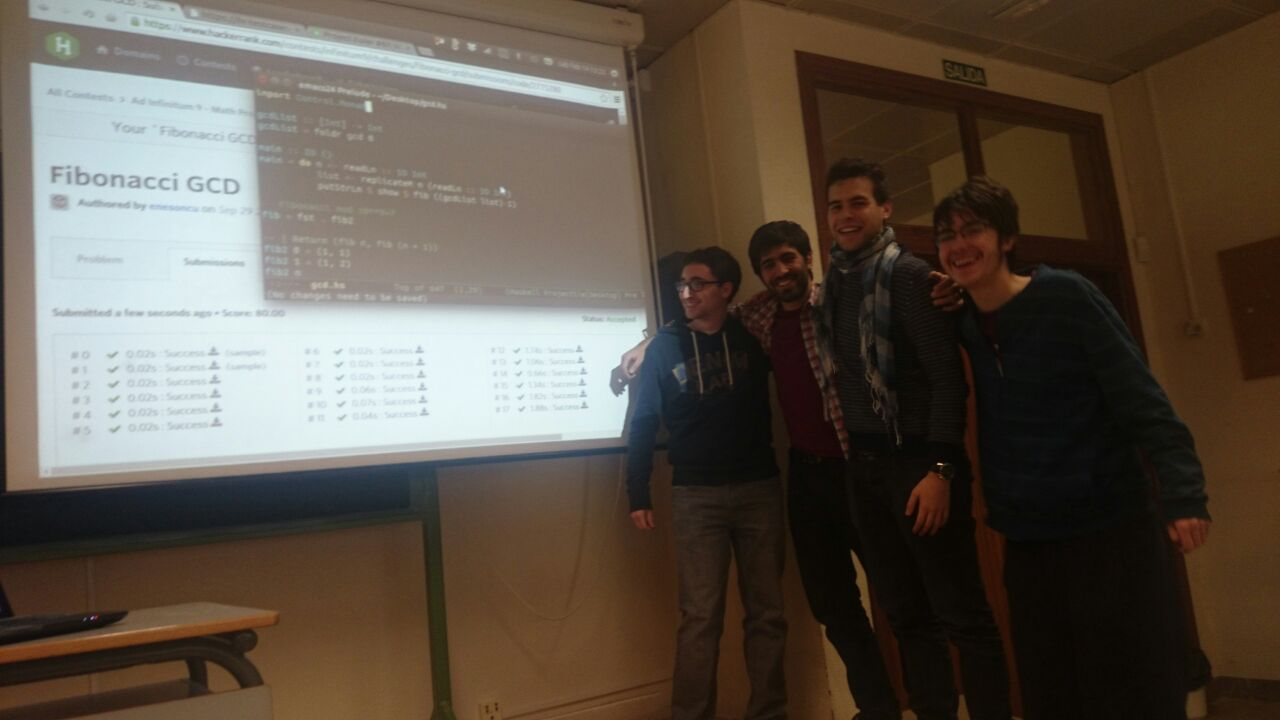
\includegraphics[width=15.5cm]{FibonacciGCD.jpg}    % -  Imagen de portada
    \vspace{1cm}
}

\author{\textbf{\autor}}                            % Autor
\date{\today}                                       % Fecha. Elija entre esta y la del título.

%----------------------------------------------------------------------------------------

\begin{document}

\maketitle

% Cambiar la etiqueta Algorithm a Algoritmo:
\makeatletter\renewcommand{\ALG@name}{Algoritmo}
\renewcommand{\listalgorithmname}{Lista de \ALG@name s} \makeatother

%----------------------------------------------------------------------------------------
%	ÍNDICE
%----------------------------------------------------------------------------------------

% Profundidad del Índice:
%\setcounter{tocdepth}{1}

\newpage
%\tableofcontents
%\newpage

%----------------------------------------------------------------------------------------
%	Problema
%----------------------------------------------------------------------------------------
\section*{Enunciado del Problema}
    El problema a resolver se encuentra en el enlace: \url{https://www.hackerrank.com/contests/infinitum9/challenges/fibonacci-gcd}. Se muestra  continuación una versión traducida del mismo.
    
    Los números de Fibbonacci tienen la siguiente forma:
    
    \begin{center}
        $F_0 = 0$\\
        $F_1 = 1$\\
        $F_2 = 1$\\
        $F_3 = 2$\\
        $\vdots$\\
        $F_n = F_{n-2} + F_{n-1}$
    \end{center}
    
    Tenemos un array $a_1,a_2,\dots,a_n$ que contiene $n$ elementos. Se pretende calcular $\gcd(F_{a_1},F_{a_2},\dots,F_{a_n})$.
    
    El formato de entrada es:
    \begin{itemize}
        \item La primera línea contiene el tamaño del array, $n$.
        \item En las siguientes $n$ líneas hay un número, la i-ésima línea contiene $a_i$.
    \end{itemize} 
    
    El formato de salida consiste en imprimir una sólo número entero. Este es el resto de la división entera del máximo común divisor pedido entre $10^9+7$.

    Las restricciones son las siguientes:
    \begin{itemize}
        \item $1 \leq n \leq 2 \times 10^5$
        \item $1 \leq a_i \leq 10^{12}$
    \end{itemize}

\section*{Solución}
    
    La primera observación a realizar es que, dado el tamaño que pueden tomar los subíndices $a_i$, no se puede pretender calcular tal cual los números de Fibonacci. Debemos obtener propiedades sobre el máximo común divisor de estos que nos permitan calcularlo de forma indirecta. La siguiente serie de proposiciones busca este objetivo. 
    
    \begin{proposition}
        Sean $n, k \in \mathbb{N}$. Se tiene que $F_{n+k} = F_{k-1}F_n + F_k F_{n+1}$. 
    \end{proposition}
    \begin{proof}
        La prueba se realiza por inducción sobre $k$ para un $n$ arbitrario en cada paso. Para $k=1$ es trivial denotando $F_0 = 0$. Supongamos el resultado cierto para $k \in \mathbb{N}$. 
        $$ F_{n+k+1} = F_{k-1}F_{n+1} + F_k F_{n+2} = F_{k-1}F_{n+1} + F_k (F_{n} + F_{n+1}) = F_{k}F_n + F_{k+1} F_{n+1} $$
        donde se ha utilizado en primer lugar la hipótesis de inducción para $k$ y posteriormente la definición de la sucesión dos veces.
    \end{proof}
    
    \begin{proposition}
        Sean $n, k \in \mathbb{N}$. Se tiene que $\gcd(F_n, F_{k+n}) = gcd(F_n, F_k)$. 
    \end{proposition}
    \begin{proof}
        En primer lugar: 
        $$ \gcd(F_n, F_{n+1}) = \gcd(F_{n}, F_{n}+F_{n-1}) = \gcd(F_{n}, F_{n-1}) $$
        donde se ha utilizado que $\gcd(a,b) = \gcd(a,b-qb)$ para cualquier $q$. Por inducción se llega a que 
        $$ \gcd(F_n, F_{n+1}) = \gcd(F_{1}, F_{2}) = \gcd(1,1) = 1 $$
        Luego los términos consecutivos de la sucesión de Fibonacci son primos relativos entre sí.
                
        Ahora, para $k > 1$ usamos la proposición anterior:
        $$ \gcd(F_n, F_{n+k}) = \gcd(F_n, F_{k-1}F_n + F_k F_{n+1}) = \gcd(F_n, F_k F_{n+1}) $$
        Como $F_n$ y $F_{n+1}$ son primos relativos:
        $$ \gcd(F_n, F_{n+k}) = \gcd(F_n, F_k F_{n+1}) = \gcd(F_n, F_k) $$
    \end{proof}
    
    \begin{proposition}
        Sean $a, b \in \mathbb{N}$. Se tiene que $\gcd(F_a, F_b) = F_{gcd(a, b)}$. 
    \end{proposition}
    \begin{proof}
        Si $a=b$ es trivial. Supongamos que $a < b$ sin pérdida de generalidad.
        Tenemos que $\gcd(F_a, F_b) = gcd(F_a, F_{b-a})$. Podemos repetir el proceso hasta que aparezca un 0 en los índices. Estamos haciendo en definitiva el Algoritmo de Euclides sobre los índices y por ser el mismo proceso tenemos garantizado que el índice final no nulo es el máximo común divisor. Esto es:
        $$ \gcd(F_a, F_b) = \gcd(F_0, F_{\gcd(a,b)}) = \gcd(0, F_{\gcd(a,b)}) = F_{\gcd(a,b)} $$
    \end{proof}
    
    \begin{proposition}
        Sean $n \in \mathbb{N}$ y $a_1, \dots a_n \in \mathbb{N}$. Se tiene que 
        $\gcd(F_{a_1}, \dots, F_{a_n}) = F_{gcd(a_1, \dots, a_n)}$. 
    \end{proposition}
    \begin{proof}
        Usaremos que $\gcd(b_1, \dots, b_n) = \gcd( \gcd(b_1, b_2), b_3, \dots, b_n)$:
        $$ \gcd(F_{a_1}, \dots, F_{a_n}) = \gcd(\gcd(F_{a_1},F_{a_2}), F_{a_3}, \dots, F_{a_n}) = \gcd(F_{\gcd(a_1, a_2)}, F_{a_3}, \dots, F_{a_n}) $$
        Repetimos el proceso $n-1$ veces y usando la definición del máximo común divisor de $n$ elementos sobre los $a_i$ obtenemos el resultado.
    \end{proof}

    De la proposición anterior se tiene automáticamente el Algoritmo \ref{algo:sol} que resuelve el problema.
    
    \begin{algorithm}
        Dados $a_1, \dots, a_n \in \{1, \dots, 10^{12}\}$ con $n \in \{1, \dots, 2\times10^5\}$. Realizamos el siguiente algoritmo:
        \begin{enumerate}
            \item Calculamos $m = \gcd(a_1, \dots, a_n)$.
            \item Calculamos $F_m \mod 10^9+7$
        \end{enumerate}
        \caption{Solución del problema GCD Fibonacci}
        \label{algo:sol}
    \end{algorithm}

    La única cuestión restante consiste en la implementación del algoritmo anterior. Para calcular el máximo común divisor de la lista utilizamos el Algoritmo de Euclides para los dos primeros elementos, que quedan sustituidos por el resultado obtenido. Repetimos el proceso hasta obtener un único número final que es el máximo común divisor buscado. Este algoritmo tiene eficiencia $n$ veces la del propio Algoritmo de Euclides. 
    
    Para calcular $F_m \mod 10^9+7$ tenemos que tener en cuenta que $m$ puede ser hasta $10^{12}$. Es fácil realizar un algoritmo lineal para este propósito calculando todos los términos progresivamente y guardando solo los dos últimos en cada iteración. Sin embargo, esto no alcanza los objetivos en el peor caso. Se propone la siguiente idea para obtener una solución logarítmica sobre $m$:
    
    \begin{equation}
        \begin{pmatrix}
            1 & 1 \\
            1 & 0 \\
        \end{pmatrix}
        \begin{pmatrix}
            F_{k+2} & F_{k+1} \\
            F_{k+1} & F_{k} \\
        \end{pmatrix}
        =
        \begin{pmatrix}
            F_{k+3} & F_{k+2} \\
            F_{k+2} & F_{k+1} \\
        \end{pmatrix}        
    \end{equation}
    
    Consecuentemente, por inducción:
    
    \begin{equation}
        \begin{pmatrix}
            1 & 1 \\
            1 & 0 \\
        \end{pmatrix}^k
        \begin{pmatrix}
            F_{2} & F_{1} \\
            F_{1} & F_{0} \\
        \end{pmatrix}
        =
        \begin{pmatrix}
            F_{k+3} & F_{k+2} \\
            F_{k+2} & F_{k+1} \\
        \end{pmatrix}        
    \end{equation}
    
    En nuestro caso:
    \begin{equation}
        \begin{pmatrix}
            F_{2} & F_{1} \\
            F_{1} & F_{0} \\
        \end{pmatrix}
        =
        \begin{pmatrix}
            1 & 1 \\
            1 & 0 \\
        \end{pmatrix}        
    \end{equation}
    Por consiguiente:
    \begin{equation}
        \begin{pmatrix}
            1 & 1 \\
            1 & 0 \\
        \end{pmatrix}^k
        =
        \begin{pmatrix}
            F_{k+2} & F_{k+1} \\
            F_{k+1} & F_{k} \\
        \end{pmatrix}        
    \end{equation}
    
    El problema se ha reducido a la exponenciación de la matriz $A =
    \begin{pmatrix} 
        1 & 1 \\ 
        1 & 0 
    \end{pmatrix}$. La exponenciación de matrices se puede conseguir logarítmica de forma análoga a la exponenciación (con exponente natural) de un número. El Algoritmo \ref{algo:exp-matrix} muestra un pseudo-código recursivo para este propósito.
    
    \begin{algorithm}
        \caption{Exponenciación de matrices. Calcula $A^n$ en $\theta(\log n)$.}
        \label{algo:exp-matrix}
        \begin{algorithmic}
            \Function{Potencia}{A, n}   
                \If{$n = 1$}  
                    \Return $A$
                \ElsIf {$n\mod{2} = 0$}
                    \State $B \gets Potencia(A,n/2)$
                    \State \Return $B^2$
                \Else
                    \State $B \gets Potencia(A,n/2)$
                    \State \Return $A B^2$                    
                \EndIf
            \EndFunction
        \end{algorithmic}
    \end{algorithm}

    Puesto que $m$ puede ser $10^12$, el resultado obtenido por el algoritmo previo puede incluso no caber en memoria. De todas formas, debemos imprimir el resultado módulo $10^9+7$. Puesto que el módulo de una suma o producto es el módulo de la suma o productos de los módulos, podemos aplicar el módulo a cada operación realizada manteniendo el mismo resultado. Los números con los que trabajará el algoritmo serán menores que $10^9+7$, pudiendo obtener el resultado sin problema.

\end{document}